% Provenance (never printed): cycle 3 "Matiere, mouvement, energie,
% information" and "La planete Terre" (meteorological phenomena, the water in
% the air, measuring the weather); see sources/book1/PROVENANCE.md.
% Book 1, grade 4, chapter 1.
\chapter{बादल, बारिश और हिम}\label{ch:g4:clouds-rain-snow}

गर्मियों की एक गरम दोपहर है। दोपहर के खाने के समय आसमान नीला था, जिसमें
रुई के गोलों जैसे कुछ छोटे सफ़ेद \omterm{def:g4:clouds-rain-snow:cloud}{बादल} थे। तीन बजते-बजते उनमें से एक बढ़ गया
है। वह ऊपर की ओर फूलता जाता है, ऊँचा और ऊँचा, किसी चपटे धूसर आधार पर खड़ी
सफ़ेद फूलगोभी की तरह। उसका सिरा फैल जाता है। उसका आधार काला पड़ जाता है।
ठंडी हवा का एक झोंका आता है, पहली मोटी बूँदें गिरती हैं, और बीस मिनट तक
मूसलाधार \omterm{def:g4:clouds-rain-snow:precipitation}{बारिश} होती है। फिर \omterm{def:g4:clouds-rain-snow:cloud}{बादल} आगे बढ़ जाता है, धूप लौट आती है, और गीले
फ़ुटपाथों से भाप उठने लगती है।

वह \omterm{def:g4:clouds-rain-snow:cloud}{बादल} कहाँ से आया? वह किस चीज़ से बना है? और उन बीस मिनटों में कितनी
\omterm{def:g4:clouds-rain-snow:precipitation}{बारिश} हुई?

\begin{recall}
किसी जगह और किसी समय पर हवा की दशा ही \omterm{def:g1:watching-the-weather:weather}{मौसम} है: धूप, \omterm{def:g4:clouds-rain-snow:cloud}{बादल}, \omterm{def:g4:clouds-rain-snow:precipitation}{बारिश}, \omterm{def:g4:clouds-rain-snow:precipitation}{हिम}, तेज़
हवा, \omterm{def:g4:clouds-rain-snow:cloud}{कोहरा}; हम उसे \omterm{def:g1:watching-the-weather:weather-chart}{मौसम-तालिका} में लिखते हैं (\cref{ch:g1:watching-the-weather})।
\omterm{def:g2:water-on-earth:ocean}{समुद्र}, \omterm{def:g1:landscapes-around-us:water}{झीलों} और ज़मीन का पानी ऊपर हवा में जाता है, और \omterm{def:g4:clouds-rain-snow:precipitation}{बारिश} बनकर वापस
नीचे आता है (\cref{ch:g2:water-on-earth})। पानी का वाष्पन (द्रव से एक अदृश्य
गैस), संघनन (गैस से फिर द्रव की नन्ही बूँदें) और जमना (द्रव से बर्फ़) कैसे
होता है, और तापमापी तापमान को डिग्री सेल्सियस में कैसे नापता है, यह भौतिकी की
पुस्तकें बताती हैं।
\end{recall}

\section{बादल क्या है?}

हमारे आसपास की हवा में हमेशा कुछ पानी होता है, एक अदृश्य गैस के रूप में:
जलवाष्प। जब हवा ऊपर उठती है, तो वह ठंडी होती है। जब वह काफ़ी ठंडी हो जाती है,
तो उसकी जलवाष्प का कुछ भाग पानी की इतनी नन्ही बूँदों में संघनित हो जाता है कि
हवा का हल्का-सा झोंका भी उन्हें तैराए रखता है। ऐसी अरबों बूँदें, एक-दूसरे से
सटकर, एक ऐसा \omterm{def:g4:clouds-rain-snow:cloud}{बादल} बनाती हैं जो हमें दिखता है। बहुत ऊपर, जहाँ हवा बहुत ठंडी
होती है, बूँदें जम जाती हैं, और \omterm{def:g4:clouds-rain-snow:cloud}{बादल} बर्फ़ के नन्हे टुकड़ों से बना होता है।

\begin{definition}[बादल और कोहरा]\label{def:g4:clouds-rain-snow:cloud}
\emph{बादल}\index{बादल} पानी की बहुत-सी नन्ही बूँदें, या बर्फ़ के बहुत-से नन्हे
टुकड़े हैं, जो हवा में एक साथ तैर रहे हैं। \emph{कोहरा}\index{कोहरा} ऐसा बादल
है जो ज़मीन को छूता है।
\end{definition}

\begin{example}[ठंडी सुबह में तुम्हारी साँस]\label{ex:g4:clouds-rain-snow:breath}
ठंडी सुबह में तुम्हारी साँस मुँह के सामने एक छोटा सफ़ेद \omterm{def:g4:clouds-rain-snow:cloud}{बादल} बना देती है।
जो हवा तुम बाहर छोड़ते हो, वह गरम होती है और उसमें जलवाष्प होती है। ठंडी हवा
उसे फ़ौरन ठंडा कर देती है, वाष्प नन्ही बूँदों में संघनित हो जाती है --- और एक
नन्हा-सा \omterm{def:g4:clouds-rain-snow:cloud}{बादल} दिखता है, जो बूँदों का फिर से वाष्पन होते ही ग़ायब हो जाता है।
\end{example}

\omterm{def:g4:clouds-rain-snow:cloud}{बादल} सफ़ेद होता है क्योंकि उसकी बूँदें सूर्य के प्रकाश को हर दिशा में बिखेर
देती हैं। जब वह बहुत घना होता है, तो उसके आधार तक थोड़ा ही प्रकाश पहुँचता है,
और नीचे से वह धूसर, या लगभग काला दिखता है: यह पानी से भरे भारी \omterm{def:g4:clouds-rain-snow:cloud}{बादल} का
संकेत है।

\section{बादलों के परिवार}

\omterm{def:g4:clouds-rain-snow:cloud}{बादल} कई आकारों के होते हैं, और दुनिया भर में \omterm{def:g1:watching-the-weather:weather}{मौसम} पर नज़र रखने वाले उन्हें
एक ही तरह से छाँटते हैं: उनके आकार से और इससे कि वे कितनी ऊँचाई पर तैरते हैं।

\begin{definition}[बादलों के परिवार]\label{def:g4:clouds-rain-snow:cloud-families}
\omterm{def:g4:clouds-rain-snow:cloud}{बादलों} के चार परिवार जानने लायक़ हैं:
\begin{itemize}
  \item \emph{कपासी मेघ}\index{कपासी मेघ}: ढेर जैसे \omterm{def:g4:clouds-rain-snow:cloud}{बादल}, सफ़ेद और फूले
        हुए, चपटे आधार वाले, रुई के गोलों जैसे;
  \item \emph{स्तरी मेघ}\index{स्तरी मेघ}: परतदार \omterm{def:g4:clouds-rain-snow:cloud}{बादल}, एक चपटी धूसर चादर
        जो नीचे रहकर पूरे आसमान को ढक लेती है;
  \item \emph{पक्षाभ मेघ}\index{पक्षाभ मेघ}: रेशेदार \omterm{def:g4:clouds-rain-snow:cloud}{बादल}, पतले सफ़ेद धागे
        या घुँघराले लच्छे, बहुत ऊँचाई पर, बर्फ़ के बने;
  \item \emph{कपासी वर्षी मेघ}\index{कपासी वर्षी मेघ}: तूफ़ानी \omterm{def:g4:clouds-rain-snow:cloud}{बादल}, एक
        विशाल मीनार जो नीचे के एक काले आधार से बहुत ज़्यादा ऊँचाई तक उठती है,
        और जिसका सिरा अक्सर चपटा होकर फैल जाता है।
\end{itemize}
\end{definition}

ये नाम \omterm{def:g4:clouds-rain-snow:cloud}{बादलों} का रूप बताते हैं: \emph{कपासी} यानी कपास जैसा ढेर, \emph{स्तरी}
यानी परत जैसा, \emph{पक्षाभ} यानी पंख जैसा, और \emph{वर्षी} यानी बरसने वाला।

\begin{omfigure}
\begin{minipage}[b]{0.49\linewidth}\centering
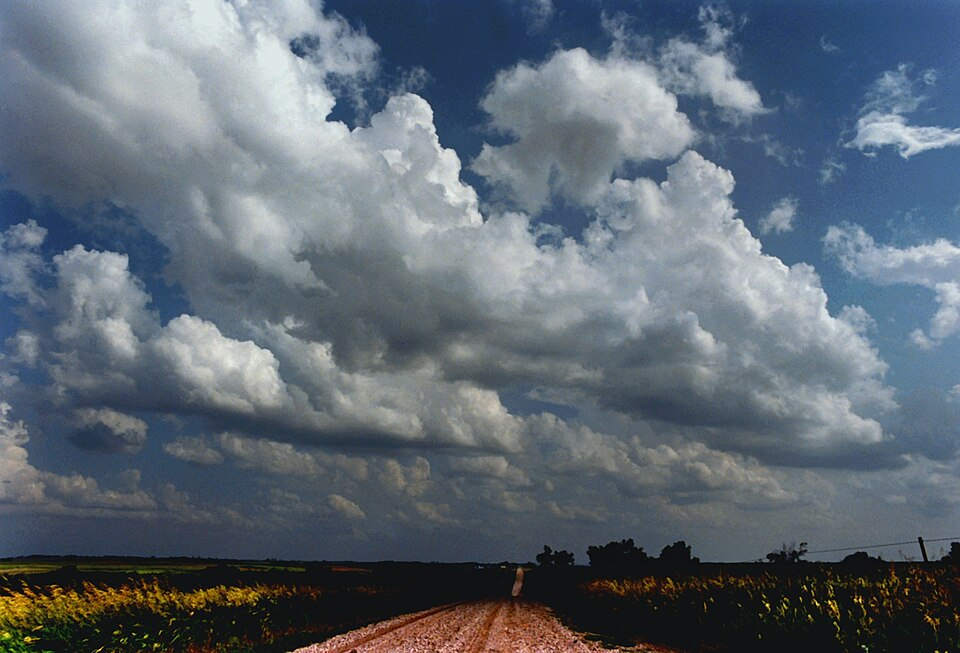
\includegraphics[width=\linewidth]{images/book1/g4-cumulus.jpg}

{\small \omterm{def:g4:clouds-rain-snow:cloud-families}{कपासी मेघ}, चपटे आधार वाले ढेर जैसे \omterm{def:g4:clouds-rain-snow:cloud}{बादल}।}
\end{minipage}\hfill
\begin{minipage}[b]{0.49\linewidth}\centering
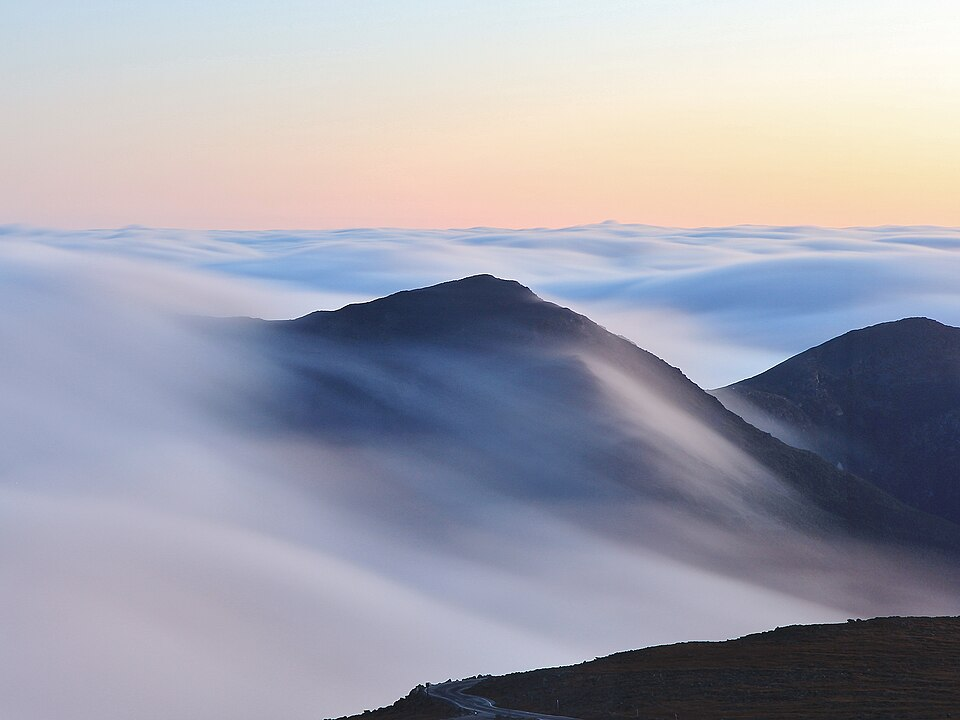
\includegraphics[width=\linewidth]{images/book1/g4-stratus.jpg}

{\small \omterm{def:g4:clouds-rain-snow:cloud-families}{स्तरी मेघ}: एक चपटी परत, जिसे यहाँ एक \omterm{def:g1:landscapes-around-us:landform}{पर्वत} से ऊपर से देखा गया है।}
\end{minipage}

\medskip
\begin{minipage}[b]{0.49\linewidth}\centering
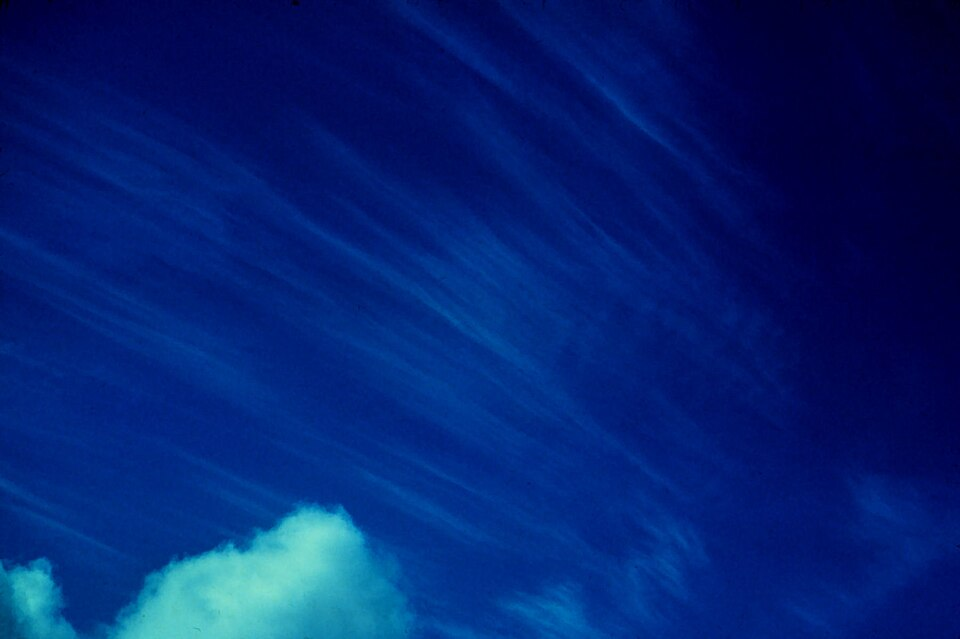
\includegraphics[width=\linewidth]{images/book1/g4-cirrus.jpg}

{\small \omterm{def:g4:clouds-rain-snow:cloud-families}{पक्षाभ मेघ}: बर्फ़ के पतले धागे, बहुत ऊँचाई पर (नीचे एक छोटा \omterm{def:g4:clouds-rain-snow:cloud-families}{कपासी मेघ})।}
\end{minipage}\hfill
\begin{minipage}[b]{0.49\linewidth}\centering
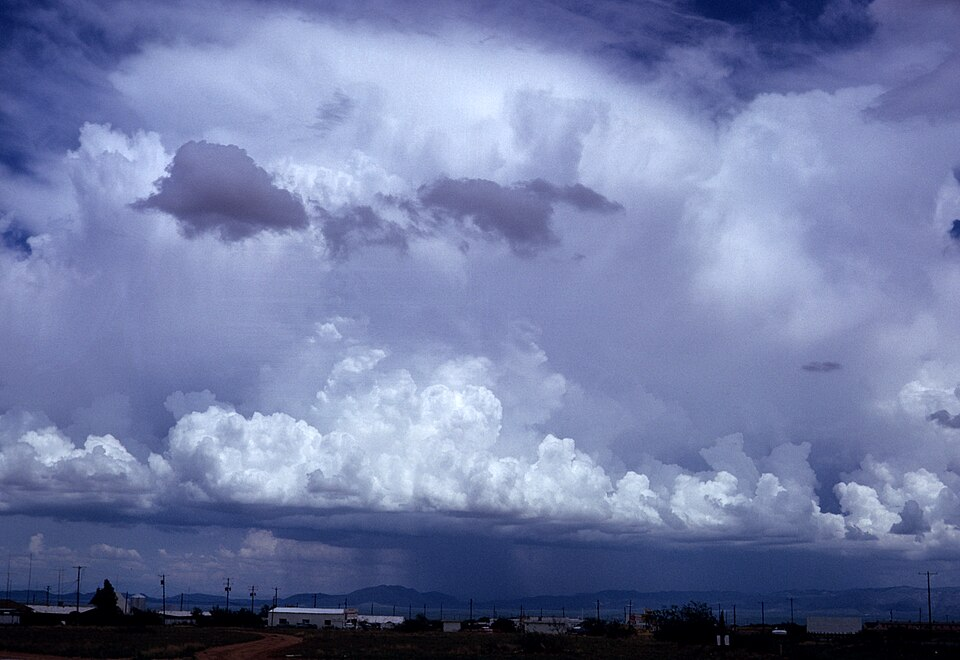
\includegraphics[width=\linewidth]{images/book1/g4-cumulonimbus.jpg}

{\small एक \omterm{def:g4:clouds-rain-snow:cloud-families}{कपासी वर्षी मेघ}: \omterm{def:g4:clouds-rain-snow:cloud}{बादल} की एक मीनार; उसके काले आधार से \omterm{def:g4:clouds-rain-snow:precipitation}{बारिश} गिर रही है।}
\end{minipage}

\smallskip
{\small चित्र: NOAA फ़ोटो लाइब्रेरी (सार्वजनिक डोमेन): एस.~कॉर्फ़िडी
(कपासी), राल्फ़ एफ़.~क्रेस्गे (पक्षाभ), बी.~हुक संग्रह (कपासी वर्षी)।}
% ledger: noaa:photos-g4
\label{fig:g4:clouds-rain-snow:photos}
\end{omfigure}

\omterm{def:g4:clouds-rain-snow:cloud}{बादल} कितनी ऊँचाई पर तैरते हैं? यह परिवार पर निर्भर करता है। नीचे के \omterm{def:g4:clouds-rain-snow:cloud}{बादल}, जैसे
\omterm{def:g4:clouds-rain-snow:cloud-families}{स्तरी मेघ} और \omterm{def:g4:clouds-rain-snow:cloud-families}{कपासी मेघ} का आधार, ज़मीन से ठीक ऊपर से लेकर लगभग 2 किलोमीटर तक
तैरते हैं। \omterm{def:g4:clouds-rain-snow:cloud-families}{पक्षाभ मेघ} बहुत ऊँचे तैरते हैं, उष्णकटिबंध और ध्रुवीय इलाक़ों के
बाहर लगभग 5 से 13 किलोमीटर के बीच --- अक्सर पृथ्वी के सबसे ऊँचे \omterm{def:g1:landscapes-around-us:landform}{पर्वत} से भी
ऊँचे।
\omterm{def:g4:clouds-rain-snow:cloud-families}{कपासी वर्षी मेघ} नीचे के आधार से लेकर \omterm{def:g4:clouds-rain-snow:cloud}{बादलों} की ऊँचाइयों के बिलकुल शीर्ष तक
फैला होता है।
% ledger: wmo:cloud-levels, wmo:cumulonimbus

\begin{omfigure}
\begin{tikzpicture}[x=1cm, y=0.5cm, font=\small]
  % height scale
  \draw[black!60] (0,0) -- (0,14);
  \foreach \h in {0,2,...,14} {
    \draw[black!60] (-0.1,\h) -- (0,\h);
    \node[anchor=east, font=\scriptsize] at (-0.12,\h) {\h\,km};
  }
  \node[anchor=south, font=\scriptsize, align=center] at (0,14.2) {ऊँचाई};
  % ground and a mountain for comparison
  \fill[green!35!black!50] (0.2,0) -- (11.4,0) -- (11.4,-0.4) -- (0.2,-0.4) -- cycle;
  \fill[black!35] (8.6,0) -- (9.9,8.8) -- (10.2,8.4) -- (11.2,0) -- cycle;
  \fill[white, draw=black!45, line width=0.3pt] (9.65,7.2) -- (9.9,8.8) -- (10.2,8.4) -- (10.4,7.0) -- (10.1,7.4) -- (9.9,7.0) -- cycle;
  \node[font=\scriptsize, align=center] at (9.9,10.2) {सबसे ऊँचा\\पर्वत};
  % levels
  \fill[blue!6] (0.2,0.15) rectangle (8.3,2);
  \fill[blue!10] (0.2,5) rectangle (8.3,13);
  \node[anchor=west, font=\scriptsize, text=blue!50!black] at (0.3,1.65) {नीचे के बादल};
  \node[anchor=west, font=\scriptsize, text=blue!50!black] at (0.3,12.6) {ऊँचे बादल};
  % stratus: a flat grey layer
  \fill[black!25, rounded corners=2pt] (0.6,0.6) rectangle (2.6,1.3);
  \node[font=\scriptsize] at (1.6,-1.1) {स्तरी};
  % cumulus
  \pic[scale=0.7, transform shape] at (4.0,0.9) {puffycloud};
  \node[font=\scriptsize] at (4.0,-1.1) {कपासी};
  % cirrus: wisps
  \foreach \y in {9.4,10.0,10.6} {
    \draw[black!50, line width=0.6pt] (0.8,\y) .. controls (1.4,\y+0.5) and (2.0,\y+0.1) .. (2.6,\y+0.6);
  }
  \node[font=\scriptsize] at (1.7,8.5) {पक्षाभ};
  % cumulonimbus: tower with an anvil
  \fill[black!15, draw=black!45, line width=0.4pt]
    (5.4,1.0) .. controls (5.2,4) and (5.6,8) .. (5.9,11.2)
    .. controls (5.0,11.6) and (4.6,12.0) .. (4.8,12.3)
    -- (8.1,12.3) .. controls (8.2,12.0) and (7.8,11.6) .. (7.0,11.2)
    .. controls (7.3,8) and (7.6,4) .. (7.4,1.0) -- cycle;
  \fill[black!45] (5.4,1.0) rectangle (7.4,1.4);
  \foreach \x in {5.7,6.1,6.5,6.9,7.2}
    \draw[omWxRain, line width=0.6pt] (\x,0.95) -- (\x-0.15,0.15);
  \node[font=\scriptsize] at (6.4,-1.1) {कपासी वर्षी};
\end{tikzpicture}

{\small \omterm{def:g4:clouds-rain-snow:cloud}{बादलों} के चारों परिवार कितनी ऊँचाई पर तैरते हैं (ऊँचाइयाँ किलोमीटर में,
उन इलाक़ों के लिए जो न उष्णकटिबंधीय हैं न ध्रुवीय)। \omterm{def:g4:clouds-rain-snow:cloud-families}{स्तरी मेघ} और \omterm{def:g4:clouds-rain-snow:cloud-families}{कपासी मेघ} का
आधार नीचे होते हैं; \omterm{def:g4:clouds-rain-snow:cloud-families}{पक्षाभ मेघ} अक्सर सबसे ऊँचे \omterm{def:g1:landscapes-around-us:landform}{पर्वत} से भी ऊँचे होते हैं।
\omterm{def:g4:clouds-rain-snow:cloud-families}{कपासी वर्षी मेघ} नीचे के आधार से \omterm{def:g4:clouds-rain-snow:cloud}{बादलों} की ऊँचाइयों के शीर्ष तक फैला होता है।
ऊँचाइयाँ विश्व \omterm{def:g1:watching-the-weather:weather}{मौसम} विज्ञान संगठन के मेघ एटलस के अनुसार।}
\label{fig:g4:clouds-rain-snow:heights}
% ledger: wmo:cloud-levels, tht:everest
\end{omfigure}

\begin{method}[बादल का नाम बताना]\label{met:g4:clouds-rain-snow:naming}
आसमान को देखो और तीन सवाल पूछो:
\begin{enumerate}
  \item क्या वह चपटे आधार वाला ढेर है? तो वह \omterm{def:g4:clouds-rain-snow:cloud-families}{कपासी मेघ} है --- और अगर वह
        उठकर एक विशाल काली मीनार बन जाए, तो \omterm{def:g4:clouds-rain-snow:cloud-families}{कपासी वर्षी मेघ}।
  \item क्या वह एक चपटी, एकसार चादर है जो पूरे आसमान को छिपा लेती है? तो वह
        \omterm{def:g4:clouds-rain-snow:cloud-families}{स्तरी मेघ} है।
  \item क्या वह बहुत ऊँचाई पर पतले सफ़ेद धागों से बना है? तो वह \omterm{def:g4:clouds-rain-snow:cloud-families}{पक्षाभ मेघ} है।
\end{enumerate}
\end{method}

\begin{remark}[बादल मौसम बताते हैं]\label{rem:g4:clouds-rain-snow:tell}
नीले आसमान में छोटे \omterm{def:g4:clouds-rain-snow:cloud-families}{कपासी मेघ} का मतलब है साफ़ \omterm{def:g1:watching-the-weather:weather}{मौसम}। धूसर \omterm{def:g4:clouds-rain-snow:cloud-families}{स्तरी मेघ} एक उदास
दिन लाता है, कभी-कभी फुहार के साथ। \omterm{def:g4:clouds-rain-snow:cloud-families}{कपासी वर्षी मेघ} छोटी, तेज़ बौछार लाता है,
अक्सर गरज, बिजली और हवा के झोंकों के साथ --- कभी-कभी \omterm{def:g4:clouds-rain-snow:precipitation}{ओले} भी। \omterm{def:g4:clouds-rain-snow:cloud-families}{पक्षाभ मेघ}
\omterm{def:g4:clouds-rain-snow:precipitation}{बारिश} नहीं लाते, पर जब वे फैलते और घने होते हैं, तो अक्सर एक दिन बाद \omterm{def:g4:clouds-rain-snow:precipitation}{बारिश}
होती है।
\end{remark}

\section{बारिश, हिम और ओले}

\omterm{def:g4:clouds-rain-snow:cloud}{बादल} के अंदर नन्ही बूँदें एक-दूसरे से टकराकर जुड़ जाती हैं, या बूँदों की क़ीमत
पर बर्फ़ के क्रिस्टल बढ़ते हैं। \omterm{def:g4:clouds-rain-snow:cloud}{बादल} की कोई बूँद, या कोई क्रिस्टल, जो काफ़ी बड़ा
और भारी हो गया हो, अब तैर नहीं पाता: वह गिर पड़ता है।

\begin{definition}[वर्षण]\label{def:g4:clouds-rain-snow:precipitation}
\emph{वर्षण}\index{वर्षण} वह पानी है जो \omterm{def:g4:clouds-rain-snow:cloud}{बादल} से ज़मीन पर गिरता है:
\emph{बारिश}\index{बारिश} (द्रव पानी की बूँदें), \emph{हिम}\index{हिम}
(आपस में चिपके बर्फ़ के क्रिस्टलों से बने फाहे) या \emph{ओले}\index{ओले}
(बर्फ़ की गोलियाँ, जो तूफ़ानी \omterm{def:g4:clouds-rain-snow:cloud}{बादलों} से गिरती हैं)।
\end{definition}

\omterm{def:g4:clouds-rain-snow:precipitation}{बारिश} होगी या \omterm{def:g4:clouds-rain-snow:precipitation}{हिम} गिरेगा, यह उस हवा के तापमान पर निर्भर करता है जिससे होकर
\omterm{def:g4:clouds-rain-snow:precipitation}{वर्षण} नीचे गिरता है। \omterm{def:g4:clouds-rain-snow:precipitation}{हिम} के फाहे ठंडे \omterm{def:g4:clouds-rain-snow:cloud}{बादल} में ऊँचाई पर बनते हैं। अगर नीचे की
हवा काफ़ी देर तक \SI{0}{\celsius} से ऊपर हो, तो वे नीचे आते-आते पिघल जाते हैं
और हम तक \omterm{def:g4:clouds-rain-snow:precipitation}{बारिश} बनकर पहुँचते हैं। अगर ज़मीन तक पूरी हवा जमा देने वाली ठंडी हो,
तो वे \omterm{def:g4:clouds-rain-snow:precipitation}{हिम} बनकर पहुँचते हैं।

\begin{omfigure}
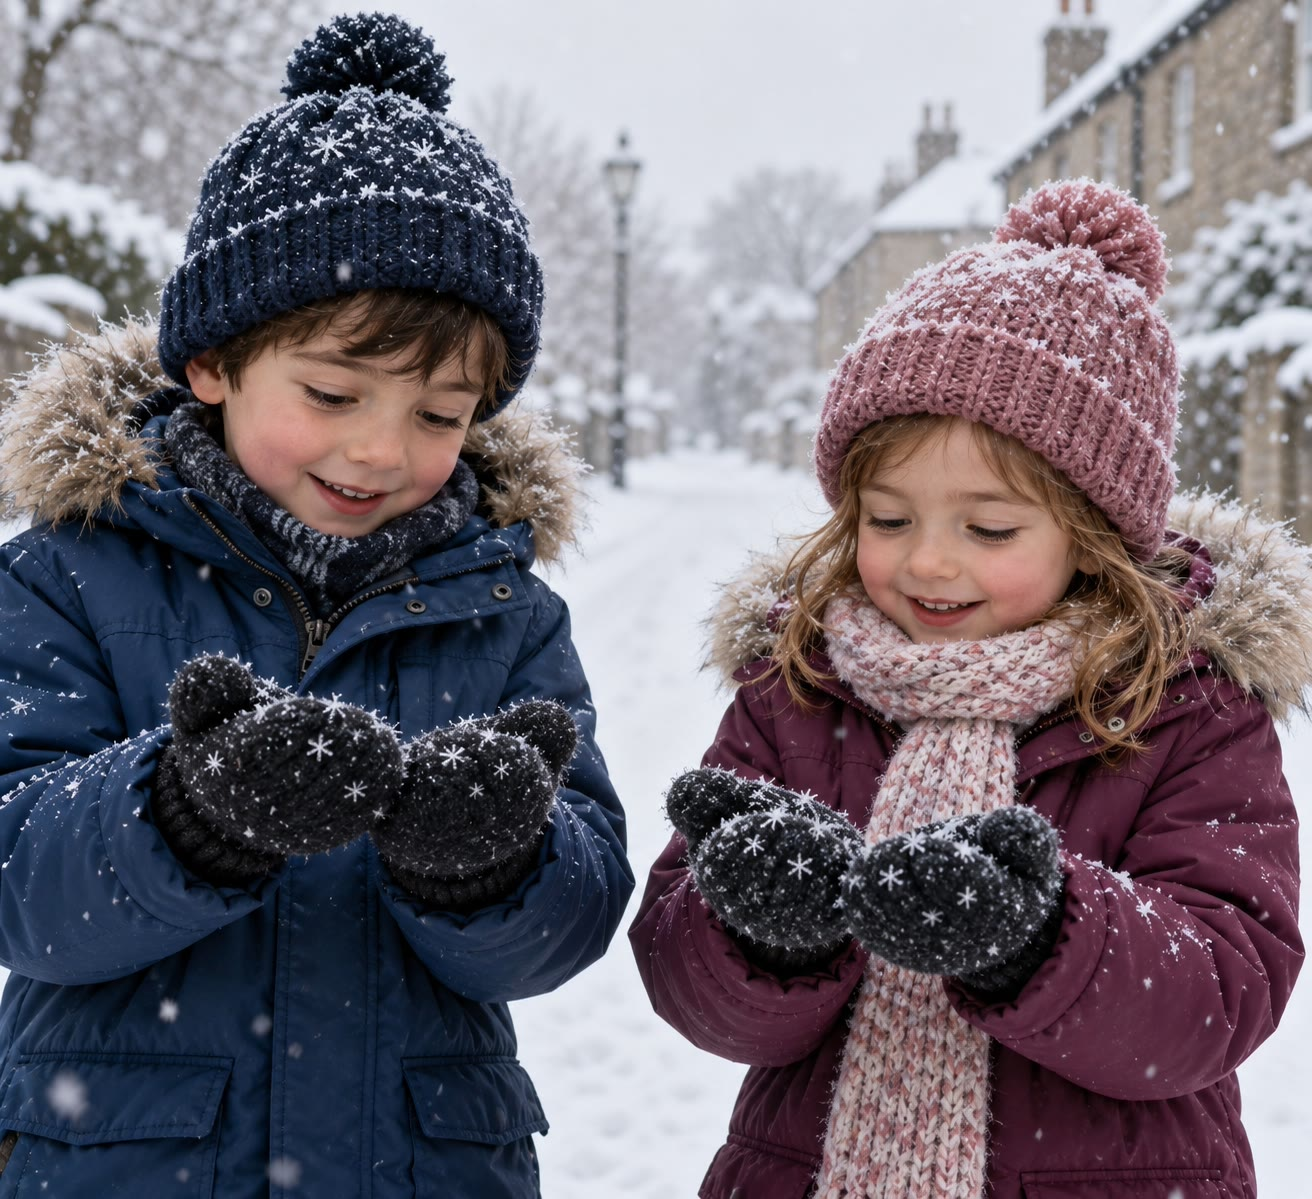
\includegraphics[width=0.55\linewidth]{images/book1/ai/g4-snowflakes.jpg}

{\small काले दस्ताने पर \omterm{def:g4:clouds-rain-snow:precipitation}{हिम} के फाहे पकड़ते बच्चे: हर फाहा बर्फ़ के क्रिस्टलों से
बना है।}
\end{omfigure}

\omterm{def:g4:clouds-rain-snow:precipitation}{ओले} सिर्फ़ \omterm{def:g4:clouds-rain-snow:cloud-families}{कपासी वर्षी मेघ} से गिरते हैं। मीनार के अंदर ऊपर की ओर चलने वाली तेज़
हवाएँ बर्फ़ की गोलियों को कई बार ऊपर-नीचे ले जाती हैं; हर चक्कर बर्फ़ की एक नई
परत जोड़ देता है, प्याज़ की परतों की तरह, जब तक ओला इतना भारी न हो जाए कि हवा
उसे थाम न सके।

\begin{omfigure}
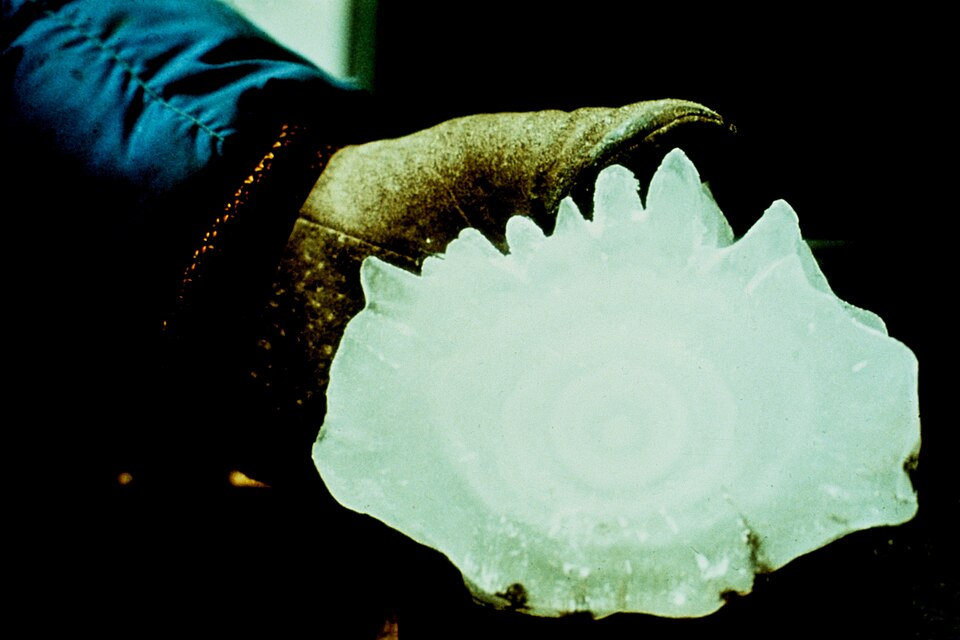
\includegraphics[width=0.5\linewidth]{images/book1/g4-hailstone.jpg}

{\small दस्ताना पहने हाथ में पकड़ा हुआ एक बहुत बड़ा ओला। छल्ले बर्फ़ की वे परतें
दिखाते हैं जो उसने तूफ़ानी \omterm{def:g4:clouds-rain-snow:cloud}{बादल} के अंदर इकट्ठा कीं। चित्र: NOAA फ़ोटो
लाइब्रेरी (सार्वजनिक डोमेन)।}
% ledger: noaa:photos-g4
\end{omfigure}

\section{मौसम को नापना}

कितनी \omterm{def:g4:clouds-rain-snow:precipitation}{बारिश} हुई, कितनी गरमी थी या हवा किधर से चली, यह बताने के लिए शब्द
काफ़ी नहीं हैं: हमें उपकरण चाहिए, और संख्याएँ।

\begin{definition}[वर्षामापी]\label{def:g4:clouds-rain-snow:rain-gauge}
\emph{वर्षामापी}\index{वर्षामापी} एक बरतन है जो अपने मुँह पर गिरने वाली \omterm{def:g4:clouds-rain-snow:precipitation}{बारिश}
को इकट्ठा करता है। उसमें इकट्ठा पानी की गहराई मिलीमीटर में नापी जाती है:
``5 मिलीमीटर \omterm{def:g4:clouds-rain-snow:precipitation}{बारिश}'' का अर्थ है कि अगर \omterm{def:g4:clouds-rain-snow:precipitation}{बारिश} का पानी न बहता और न ज़मीन में
रिसता, तो समतल ज़मीन पर पानी की 5 मिलीमीटर गहरी परत बन जाती।
\end{definition}

\begin{remark}[एक मिलीमीटर बारिश बहुत पानी है]\label{rem:g4:clouds-rain-snow:litre}
\omterm{def:g4:clouds-rain-snow:rain-gauge}{वर्षामापी} में एक मिलीमीटर \omterm{def:g4:clouds-rain-snow:precipitation}{बारिश} बहुत थोड़ी दिखती है। पर एक मीटर गुणा एक मीटर
के ज़मीन के वर्ग पर यह एक लीटर पानी है: एक बड़ी बोतल। एक हज़ार वर्ग मीटर के
स्कूल के मैदान पर 10 मिलीमीटर की \omterm{def:g4:clouds-rain-snow:precipitation}{बारिश} दस हज़ार लीटर पानी लाती है: 10-10 लीटर
की एक हज़ार बाल्टियाँ भरने के लिए काफ़ी।
\end{remark}

\begin{omfigure}
\begin{tikzpicture}[font=\small]
  % funnel
  \draw[black!70, line width=0.8pt] (-1.2,6.6) -- (-0.35,5.8) -- (-0.35,5.4);
  \draw[black!70, line width=0.8pt] (1.2,6.6) -- (0.35,5.8) -- (0.35,5.4);
  \draw[black!70, line width=0.8pt] (-1.2,6.6) -- (1.2,6.6);
  % tube
  \fill[blue!25] (-0.45,0) rectangle (0.45,2.4);
  \draw[black!70, line width=0.8pt] (-0.45,5.4) -- (-0.45,0) -- (0.45,0) -- (0.45,5.4);
  \foreach \m in {0,1,...,50} {
    \pgfmathsetmacro{\yy}{\m*0.1}
    \draw[black!60] (0.45,\yy) -- ++(-0.12,0);
  }
  \foreach \m in {0,5,10,...,50} {
    \pgfmathsetmacro{\yy}{\m*0.1}
    \draw[black!80] (0.45,\yy) -- ++(-0.25,0);
    \node[anchor=west, font=\scriptsize] at (0.5,\yy) {\m};
  }
  \node[anchor=west, font=\scriptsize] at (1.0,5.0) {मिमी};
  % reading line
  \draw[red!70!black, -{Stealth}] (-1.6,2.4) -- (-0.5,2.4);
  \node[anchor=east, align=right, font=\scriptsize] at (-1.65,2.4) {स्तर यहाँ\\पढ़ो};
  \node[anchor=west, font=\scriptsize] at (1.9,2.4) {$\leftarrow$ 24\,मिमी बारिश};
\end{tikzpicture}

{\small एक सरल \omterm{def:g4:clouds-rain-snow:rain-gauge}{वर्षामापी}: एक कीप \omterm{def:g4:clouds-rain-snow:precipitation}{बारिश} को पकड़ती है और मिलीमीटर में निशान
लगी एक नली उसे थामती है। पानी का स्तर अपनी आँख को उसी ऊँचाई पर रखकर पढ़ो।
यहाँ, पिछली बार \omterm{def:g4:clouds-rain-snow:rain-gauge}{वर्षामापी} ख़ाली करने के बाद से 24 मिलीमीटर \omterm{def:g4:clouds-rain-snow:precipitation}{बारिश} हुई है।}
\label{fig:g4:clouds-rain-snow:gauge}
\end{omfigure}


\begin{definition}[वायु-दिशासूचक]\label{def:g4:clouds-rain-snow:wind-vane}
\emph{वायु-दिशासूचक}\index{वायु-दिशासूचक} एक तीर है जो किसी खंभे पर आज़ादी से
घूमता है। हवा उसकी पूँछ को धकेलती है, इसलिए तीर हमेशा उस दिशा की ओर इशारा
करता है जिधर \emph{से} हवा आ रही है।
\end{definition}

\begin{definition}[मौसम केंद्र]\label{def:g4:clouds-rain-snow:weather-station}
\emph{मौसम केंद्र}\index{मौसम केंद्र} वह जगह है जहाँ हर दिन, हमेशा एक ही
तरीक़े से, उपकरणों से \omterm{def:g1:watching-the-weather:weather}{मौसम} नापा जाता है: हवादार सफ़ेद बक्से में एक तापमापी,
खुली जगह में एक \omterm{def:g4:clouds-rain-snow:rain-gauge}{वर्षामापी}, और एक खंभे पर \omterm{def:g4:clouds-rain-snow:wind-vane}{वायु-दिशासूचक}।
\end{definition}

तापमापी को छाया में, झिलमिलीदार दीवारों वाले एक सफ़ेद बक्से में रखा जाता है,
जो हवा को अंदर आने देता है पर धूप और \omterm{def:g4:clouds-rain-snow:precipitation}{बारिश} को रोकता है। यूनाइटेड किंगडम की
\omterm{def:g1:watching-the-weather:weather}{मौसम} सेवा, मेट ऑफ़िस, उसे ज़मीन से \SI{1.25}{\metre} ऊपर रखती है। \omterm{def:g4:clouds-rain-snow:rain-gauge}{वर्षामापी}
खुली जगह में खड़ा होता है, उन दीवारों और पेड़ों से दूर जो उसे \omterm{def:g4:clouds-rain-snow:precipitation}{बारिश} से बचा लेते,
और उसका मुँह ज़मीन से थोड़ा ऊपर होता है। \omterm{def:g4:clouds-rain-snow:wind-vane}{वायु-दिशासूचक} अपने खंभे पर ऊँचा लगा
होता है, उन रुकावटों के ऊपर जो हवा की दिशा मोड़ देतीं।
% ledger: mo:screen-height, mo:raingauge

\begin{omfigure}
\begin{tikzpicture}[font=\small, x=1cm, y=1cm]
  % grass
  \fill[green!40!black!45] (-0.5,0) rectangle (11,-0.25);
  \foreach \x in {-0.3,0.1,...,10.8} \draw[green!45!black] (\x,0) -- ++(0.06,0.14);
  % screen on legs
  \draw[black!70, line width=1pt] (0.8,0) -- (0.8,1.25) (2.2,0) -- (2.2,1.25);
  \fill[white, draw=black!70] (0.6,1.25) rectangle (2.4,2.4);
  \foreach \y in {1.4,1.55,...,2.25} \draw[black!40] (0.7,\y) -- (2.3,\y-0.08);
  \fill[white, draw=black!70] (0.45,2.4) -- (1.5,2.75) -- (2.55,2.4) -- cycle;
  \draw[black!60, <->] (2.8,0) -- node[right, font=\scriptsize, align=left] {लगभग\\1.25\,m} (2.8,1.25);
  \node[align=center, font=\scriptsize] at (1.5,3.25) {सफ़ेद झिलमिलीदार\\बक्से में तापमापी};
  % rain gauge
  \fill[black!15, draw=black!70] (5.4,0) rectangle (5.9,0.4);
  \draw[black!70] (5.3,0.55) -- (5.4,0.4) (6.0,0.55) -- (5.9,0.4);
  \node[align=center, font=\scriptsize] at (5.65,1.2) {वर्षामापी,\\खुली जगह में};
  % tree far away
  \fill[brown!60!black] (7.3,0) rectangle (7.5,1.3);
  \fill[green!50!black!70] (7.4,2.1) circle (0.85);
  % wind vane on a mast
  \draw[black!70, line width=1pt] (9.8,0) -- (9.8,4.2);
  \draw[black!80, line width=1.4pt, -{Latex[length=3mm]}] (10.6,4.4) -- (9.0,4.4);
  \fill[black!80] (10.6,4.4) -- (10.9,4.65) -- (10.9,4.15) -- cycle;
  \node[align=center, font=\scriptsize] at (9.8,5.05) {ऊँचे खंभे पर वायु-दिशासूचक};
  \node[anchor=west, font=\scriptsize, align=left] at (10.1,3.4) {उधर इशारा करता है\\जिधर से हवा आती है};
\end{tikzpicture}

{\small एक छोटा \omterm{def:g4:clouds-rain-snow:weather-station}{मौसम केंद्र}। तापमापी छाया में, झिलमिलीदार दीवारों वाले एक सफ़ेद
बक्से में, घास से लगभग 1.25 मीटर ऊपर है; \omterm{def:g4:clouds-rain-snow:rain-gauge}{वर्षामापी} खुली जगह में, पेड़ से दूर
खड़ा है; \omterm{def:g4:clouds-rain-snow:wind-vane}{वायु-दिशासूचक} रुकावटों से बहुत ऊपर है।}
\label{fig:g4:clouds-rain-snow:station}
% ledger: mo:screen-height
\end{omfigure}

\begin{inthefield}[स्कूल के आँगन में मौसम केंद्र]
बहुत-से स्कूल खेल के मैदान के एक कोने में एक छोटा \omterm{def:g4:clouds-rain-snow:weather-station}{मौसम केंद्र} रखते हैं। हर
सुबह एक ही समय पर दो विद्यार्थी तापमापी पढ़ते हैं, \omterm{def:g4:clouds-rain-snow:rain-gauge}{वर्षामापी} पढ़कर उसे ख़ाली
करते हैं, और लिखते हैं कि \omterm{def:g4:clouds-rain-snow:wind-vane}{वायु-दिशासूचक} किधर इशारा कर रहा है। हफ़्तों में कक्षा
अपने \omterm{def:g1:watching-the-weather:weather}{मौसम} का अपना एक रिकॉर्ड बना लेती है।
\end{inthefield}

\begin{omfigure}
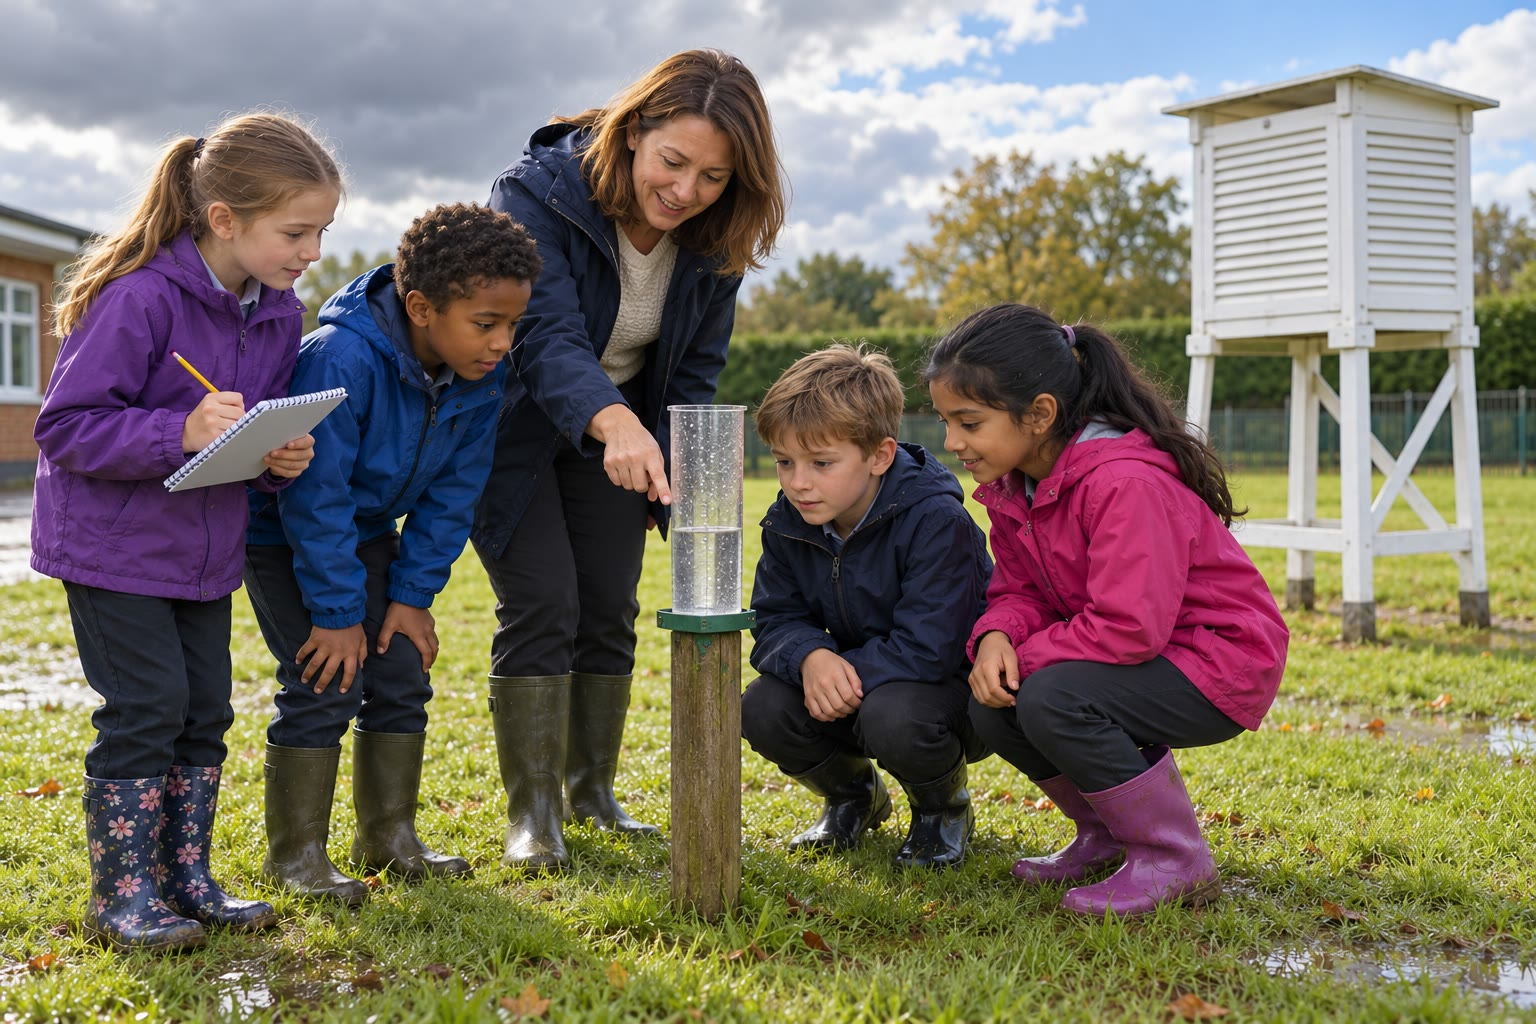
\includegraphics[width=0.55\linewidth]{images/book1/ai/g4-rain-gauge-class.jpg}

{\small स्कूल के आँगन में \omterm{def:g4:clouds-rain-snow:rain-gauge}{वर्षामापी} पढ़ते विद्यार्थी।}
\end{omfigure}

\begin{method}[बारिश का दंड आलेख बनाना]\label{met:g4:clouds-rain-snow:bar-chart}
एक हफ़्ते की \omterm{def:g4:clouds-rain-snow:precipitation}{बारिश} का चित्र बनाने के लिए:
\begin{enumerate}
  \item एक क्षैतिज रेखा खींचो और उसके नीचे बराबर दूरी पर दिन लिखो;
  \item बाईं ओर एक ऊर्ध्वाधर रेखा खींचो और उस पर बराबर क़दमों में (जैसे हर
        2 मिलीमीटर पर) मिलीमीटर के निशान लगाओ;
  \item हर दिन के ऊपर उस दिन की \omterm{def:g4:clouds-rain-snow:precipitation}{बारिश} जितना ऊँचा एक दंड बनाओ; जिस दिन \omterm{def:g4:clouds-rain-snow:precipitation}{बारिश}
        नहीं हुई, उसका कोई दंड नहीं बनता;
  \item आलेख को एक शीर्षक दो और ऊर्ध्वाधर रेखा पर मात्रक, मिमी, लिखो।
\end{enumerate}
\end{method}

\begin{example}[स्कूल में बारिश का एक हफ़्ता]\label{ex:g4:clouds-rain-snow:week}
कक्षा ने एक हफ़्ते तक हर सुबह \omterm{def:g4:clouds-rain-snow:rain-gauge}{वर्षामापी} पढ़ा और यह पाया: सोमवार 0, मंगलवार 4,
बुधवार 12, गुरुवार 7, शुक्रवार 0, शनिवार 2, रविवार 5 मिलीमीटर। सबसे गीला दिन
बुधवार था। सोमवार और शुक्रवार को \omterm{def:g4:clouds-rain-snow:precipitation}{बारिश} नहीं हुई। पूरे हफ़्ते में
$0 + 4 + 12 + 7 + 0 + 2 + 5 = 30$ मिलीमीटर \omterm{def:g4:clouds-rain-snow:precipitation}{बारिश} हुई। अकेले बुधवार ने 30 में
से 12 मिलीमीटर दिए, यानी हफ़्ते की \omterm{def:g4:clouds-rain-snow:precipitation}{बारिश} का $\frac{12}{30} = \frac{2}{5}$।
\end{example}

\begin{omfigure}
\begin{tikzpicture}
\begin{axis}[ybar, bar width=14pt, width=0.8\linewidth, height=5.4cm,
    ymin=0, ymax=14, ytick={0,2,...,14}, ylabel={बारिश (मिमी)},
    symbolic x coords={Mon,Tue,Wed,Thu,Fri,Sat,Sun}, xtick=data,
    xticklabels={सोम,मंगल,बुध,गुरु,शुक्र,शनि,रवि},
    axis x line*=bottom, axis y line*=left, ymajorgrids, grid style={gray!25},
    nodes near coords, nodes near coords style={font=\scriptsize},
    every axis label/.append style={font=\small}, tick label style={font=\small},
    title={स्कूल में बारिश, एक हफ़्ता}, title style={font=\small}]
  \addplot[fill=omWxRain!70, draw=omWxRain!60!black] coordinates
    {(Mon,0) (Tue,4) (Wed,12) (Thu,7) (Fri,0) (Sat,2) (Sun,5)};
\end{axis}
\end{tikzpicture}

{\small \cref{ex:g4:clouds-rain-snow:week} वाला हफ़्ता दंड आलेख के रूप में।}
\label{fig:g4:clouds-rain-snow:bars}
\end{omfigure}

\section{अभ्यास}

\begin{exercise}[$\star$]\label{exo:g4:clouds-rain-snow:1}
\omterm{def:g4:clouds-rain-snow:cloud}{बादल} किससे बना होता है? \omterm{def:g4:clouds-rain-snow:cloud}{कोहरा} क्या है?
\end{exercise}

\begin{exercise}[$\star$]\label{exo:g4:clouds-rain-snow:2}
\omterm{def:g4:clouds-rain-snow:cloud}{बादल} का नाम बताओ: (क) एक चपटी धूसर चादर जो पूरे आसमान को छिपा लेती है;
(ख) नीले आसमान में बहुत ऊँचे पतले सफ़ेद धागे; (ग) रुई जैसे, चपटे आधार वाले सफ़ेद
ढेर; (घ) चपटे सिरे वाली एक विशाल काली मीनार, जो गरज लाती है।
\end{exercise}

\begin{exercise}[$\star$]\label{exo:g4:clouds-rain-snow:3}
\omterm{def:g4:clouds-rain-snow:precipitation}{बारिश}, \omterm{def:g4:clouds-rain-snow:precipitation}{हिम} या \omterm{def:g4:clouds-rain-snow:precipitation}{ओले}? (क) तूफ़ानी \omterm{def:g4:clouds-rain-snow:cloud}{बादल} से गिरने वाली बर्फ़ की गोलियाँ; (ख) द्रव
पानी की बूँदें; (ग) बर्फ़ के क्रिस्टलों से बने फाहे।
\end{exercise}

\begin{exercise}[$\star$]\label{exo:g4:clouds-rain-snow:4}
कौन-सा उपकरण नापता है: (क) \omterm{def:g4:clouds-rain-snow:precipitation}{बारिश}; (ख) तापमान; (ग) हवा किधर से आती है?
\end{exercise}

\begin{exercise}[$\star$]\label{exo:g4:clouds-rain-snow:5}
पृष्ठ~\pageref{fig:g4:clouds-rain-snow:gauge} पर बने \omterm{def:g4:clouds-rain-snow:rain-gauge}{वर्षामापी} में पानी अब 17 के
निशान तक पहुँचता है। कितने मिलीमीटर \omterm{def:g4:clouds-rain-snow:precipitation}{बारिश} हुई है? इसे 20 तक पहुँचाने के लिए
कितने मिलीमीटर और चाहिए?
\end{exercise}

\begin{exercise}[$\star$]\label{exo:g4:clouds-rain-snow:6}
पृष्ठ~\pageref{fig:g4:clouds-rain-snow:bars} का दंड आलेख देखो। सबसे गीला दिन
कौन-सा था? किन दिनों \omterm{def:g4:clouds-rain-snow:precipitation}{बारिश} नहीं हुई? किस दिन 7 मिलीमीटर \omterm{def:g4:clouds-rain-snow:precipitation}{बारिश} हुई?
\end{exercise}

\begin{exercise}[$\star\star$]\label{exo:g4:clouds-rain-snow:7}
\omterm{def:g4:clouds-rain-snow:precipitation}{हिम} वाले एक दिन की सुबह \omterm{def:g1:landscapes-around-us:landform}{पहाड़ी} गाँव में \omterm{def:g4:clouds-rain-snow:precipitation}{हिम} के फाहे ज़मीन तक पहुँचते हैं, पर
नीचे \omterm{def:g1:landscapes-around-us:landform}{घाटी} में \omterm{def:g4:clouds-rain-snow:precipitation}{बारिश} होती है। हवा के तापमान की मदद से यह अंतर समझाओ।
\end{exercise}

\begin{exercise}[$\star\star$]\label{exo:g4:clouds-rain-snow:8}
एक और हफ़्ते कक्षा यह पाती है: सोमवार 3, मंगलवार 0, बुधवार 1, गुरुवार 9,
शुक्रवार 6, शनिवार 0, रविवार 1 मिलीमीटर। दंड आलेख बनाओ। हफ़्ते में कितने
मिलीमीटर \omterm{def:g4:clouds-rain-snow:precipitation}{बारिश} हुई? हफ़्ते की \omterm{def:g4:clouds-rain-snow:precipitation}{बारिश} का कितना भाग गुरुवार को गिरा?
\end{exercise}

\begin{exercise}[$\star\star$]\label{exo:g4:clouds-rain-snow:9}
\omterm{def:g4:clouds-rain-snow:rain-gauge}{वर्षामापी} खुली जगह में, दीवारों और पेड़ों से दूर क्यों होना चाहिए? तापमापी को
छाया में एक सफ़ेद बक्से में क्यों रखा जाता है, सीधी धूप में क्यों नहीं?
\end{exercise}

\begin{exercise}[$\star\star$]\label{exo:g4:clouds-rain-snow:10}
\omterm{def:g4:clouds-rain-snow:wind-vane}{वायु-दिशासूचक} पश्चिम की ओर इशारा करता है। हवा किधर से आ रही है? वह किधर जा
रही है?
\end{exercise}

\begin{exercise}[$\star\star\star$]\label{exo:g4:clouds-rain-snow:11}
500 वर्ग मीटर के एक मैदान पर 8 मिलीमीटर \omterm{def:g4:clouds-rain-snow:precipitation}{बारिश} होती है।
\cref{rem:g4:clouds-rain-snow:litre} की मदद से बताओ कि मैदान पर कितने लीटर
पानी गिरा। एक झारी में 10 लीटर पानी आता है: यह कितनी झारियाँ हुईं?
\end{exercise}
